\documentclass[documentation.tex]{subfiles}
\begin{document}
\subsection{Circuito}
		Viene riportato di seguito il circuito che si trova all'interno del
		giocattolo:
		
		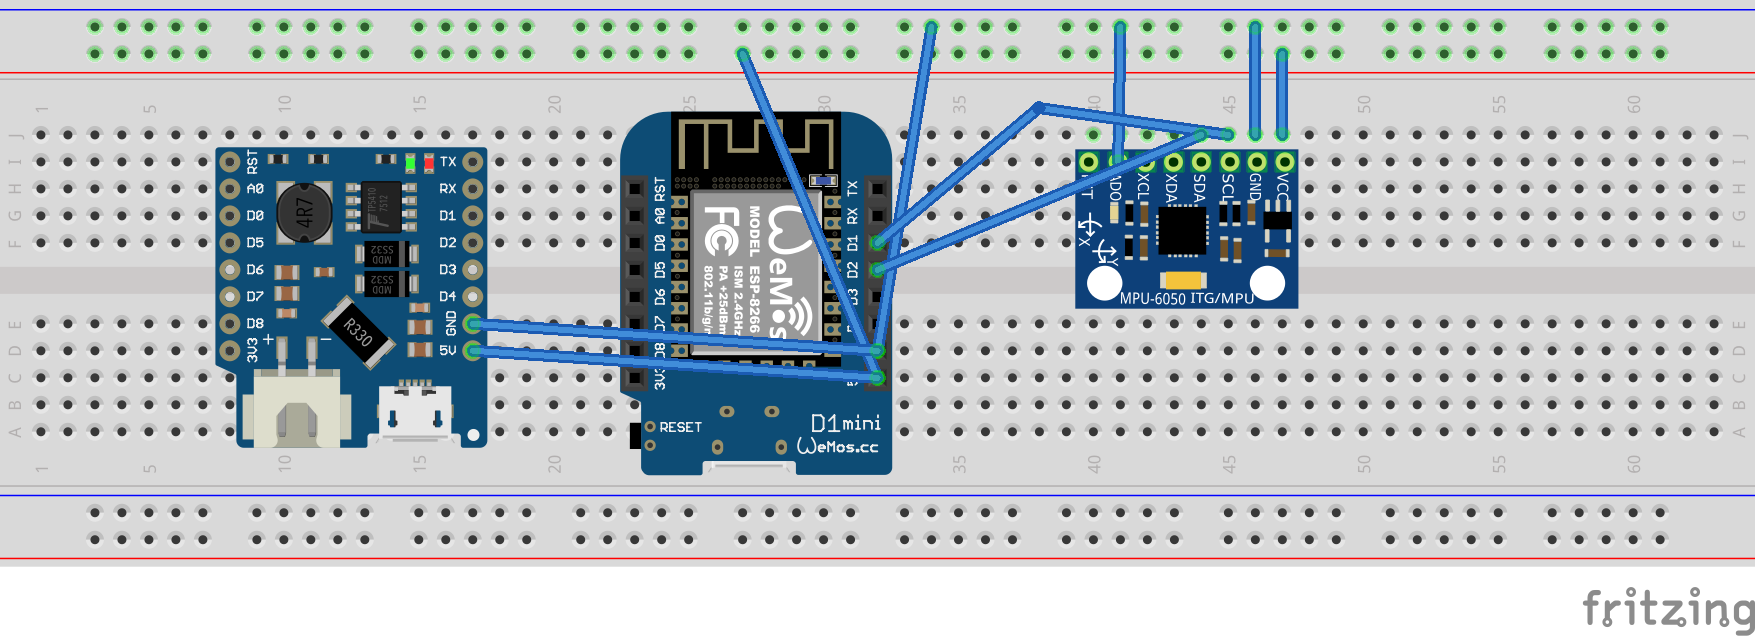
\includegraphics[width=\textwidth]{./images/circuit.png}
		
		Le componenti del circuito sono:
		\begin{itemize}
			\item Wemos D1 mini
			\item MPU-6050, accelerometro a 6 assi
			\item Wemos Battery Shield
		\end{itemize}
		\subsection{Cablaggio}
		\begin{tabular}{|c|c|}
			\hline
			\textbf{Battery Shield} & \textbf{D1 mini} \\
			\hline
			5V & 5V \\ \hline
			GND & G \\ \hline		
		\end{tabular}
		\begin{tabular}{|c|c|}
			\hline
			\textbf{D1 mini} & \textbf{MPU-6050} \\
			\hline
			5V & VCC \\ \hline
			G & GND \\ \hline
			D1(SCL) & SCL \\ \hline
			D2(SDA) & SDA \\ \hline
			G & AD0 \\ \hline		
		\end{tabular}
		\subsection{Descrizione}
		\begin{itemize}
		\item La componente MPU-6050 è in grado di misurare l'accelerazione della scheda lungo gli assi x,y,z. Tale accelerazione è proporzionale alla somma vettoriale di tutte le forze applicate. Nel progetto il sensore viene utilizzato per fare motion detection, cioè le accelerazioni misurate vengono rielaborate per decidere se la scheda(e il giocattolo di conseguenza) viene spostata lungo una certa direzione: in particolare, se la scheda viene mossa lungo una certa direzione con un certo verso, il sensore misurerà un'accelerazione di una intensità proporzionale alla forza appplicata lungo tali direzione e verso(proiettata lungo gli assi x, y, z su cui avvengono le misurazioni). Dati gli inevitabili errori di misura dello strumento, i dati raccolti e inviati dal circuito verranno sottoposti all'azione filtrante di un filtro passa-basso(vedi sezione software).
		\item La scheda Wemos D1 mini, oltre a fornire il microcontrollore che esegue lo sketch riportato nella sezione software, viene usato come Access Point creando una rete internet ad-hoc. Il videogioco si connette alla scheda generando una connessione TCP al momento della generazione del percorso. Il D1 mini si comporta quindi da server inviando le misure ottenute dall'accelerometro al videogioco.
		\item La Wemos Battery Shield consente di alimentare il circuito usando una batteria al litio, di dimensioni ridotte e ricaricabile.
		\end{itemize}
\end{document}